\chapter{Security of network applications}
\section{Standard situation}
The standard situation for an ordinary network application is very \textbf{negative}, since most of the systems implement very \textbf{weak authN mechanism} that typically rely on \texttt{username} and \texttt{password}, which can lead to:
\begin{itemize}
    \item Password Snooping
    \item IP Spoofing 
\end{itemize}
Even if \textbf{stronger authN mechanism} is implemented, there are still problems with data:
\begin{itemize}
    \item Data Snooping/Forging
    \item Shadow Server/MITM
    \item Replay and Filtering attacks
\end{itemize}
So to resolve these problems, we can use two different approaches: \textbf{Channel Security} and \textbf{Message/Data Security}.

\section{Channel Security}
\begin{minipage}{0.7\textwidth}
%	\vspace{-0.5cm}
Channel Security implements a secure connection between two nodes. To achieve this, before the start of the communication, the two nodes need to negotiate the \texttt{algorithms}, \texttt{parameters} and \texttt{keys} to protect the whole traffic that will be sent through the communication channel.
\end{minipage} 
\hspace{0.5cm}
\begin{minipage}{0.3\textwidth}
    \centering
    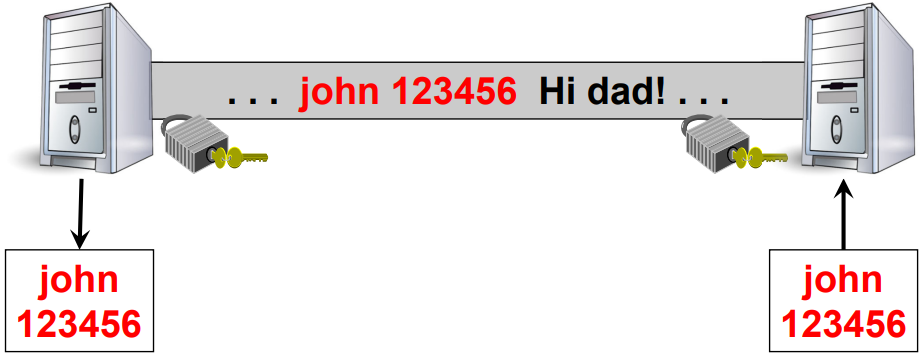
\includegraphics[width=\textwidth]{/home/lorenzo/Notes/Information System Security/images/Screenshot from 2024-12-22 13-22-37.png}
\end{minipage}
\noindent
Since all this features are negotiated \textbf{before transmitting data}, we ensure:
\begin{itemize}
    \item \textbf{Single} or \textbf{mutual authN}
    \item \textbf{Data integrity}
    \item \textbf{Data confidentiality}
\end{itemize}
Channel Security is very easy to implement because it requires no (or small) modification of applications. Since this features are also negotiated \textbf{automatically} we cannot have \textbf{non-repudation}.\\
\\
\textcolor{red}{\textbf{N.B.}} The \textbf{main issue} with Channel Security is that its security properties are provided \textbf{only} during the transit \textbf{inside} the communication channel. So data in \textbf{not} protected when it's located at the end-user. 

\section{Message/Data security}
\begin{minipage}{0.6\textwidth}
%	\vspace{-0.5cm}
It applies protection \textbf{only} when it's needed. This means that data is \textbf{individually} protected by wrapping it into a \textbf{secure container}. Data (not the channel) ensures the following security properties:
\begin{itemize}
    \item \textbf{Single authN, not mutual} because features are \textbf{not negotiated}
    \item \textbf{Data integrity}
    \item \textbf{Data confidentiality}
\end{itemize}
\end{minipage} 
\hspace{0.5cm}
\begin{minipage}{0.4\textwidth}
    \centering
    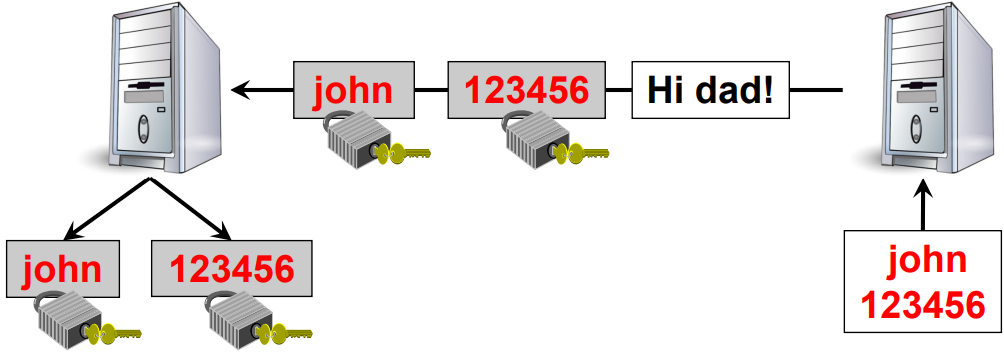
\includegraphics[width=\textwidth]{/home/lorenzo/Pictures/Screenshots/Screenshot from 2024-12-22 13-44-53.png}
\end{minipage}
\noindent
\newline
\\If protection is applied \textbf{voluntary} and \textbf{explicity} by the user, we can have \textbf{non-repudation}. Message/Data Security requires modification to application.
\newpage
\section{Different implementation}
\texttt{Channel Security} and \texttt{Message/Data Security} can be \textbf{combined} in order to get the \textbf{benefits} of both. These security concepts can be  implemented in two different way:
\\
\newline
\begin{minipage}{0.5\textwidth}
    \subsubsection{Security Internal to Applications}
    \begin{center}
        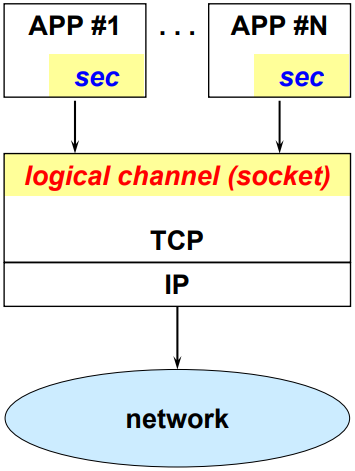
\includegraphics[width=0.3\textwidth]{/home/lorenzo/Notes/Information System Security/images/Screenshot from 2024-12-22 15-33-07.png}
    \end{center}
    In this approach \textbf{each application implements security internally}. The common part is limited to the communication channels (socket). They could be:
    \begin{itemize}
        \item  \textbf{Possible implementation errors} (implementing security protocols is not simple)
        \item Does not guarantee interoperability (-> security specification could be different between applications)
    \end{itemize}
    \textcolor{red}{\textbf{N.B.}} \textbf{Communication channels} are the \textbf{only} common part between the various application application and are used to exchange information.
\end{minipage} 
\hspace{0.5cm}
\begin{minipage}{0.5\textwidth}
    \vspace{-1cm}
    \subsubsection{Security External to Applications}
    \begin{center}
        \centering
        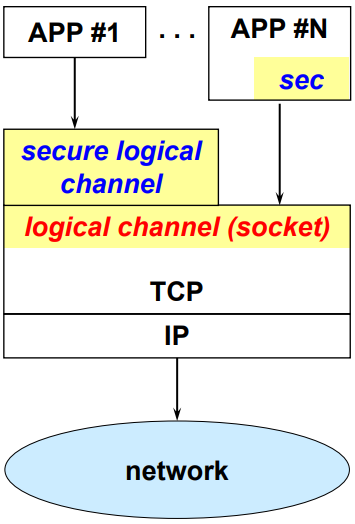
\includegraphics[width=0.3\textwidth]{/home/lorenzo/Notes/Information System Security/images/Screenshot from 2024-12-22 16-57-52.png}
    \end{center}
    A \textbf{Secure Socket} is created on top of the already existing "normal" socket, effectively creating a \textbf{new level} called \textbf{Secure Session Level (SSL)}. The Secure Socket implements all the security functio3.12.1 Web-Based Payment Systems
    The steps are:
    1. The merchant M presents the products or services on their website
    for the carholder C to browser.
    2. C places an order through the merchant’s website, initiating the pay-
    ment process.
    3. M redirects C to a payment gateway PG.
    4. PG will create a Secure TLS channel between the PG itself and C.
    5. C provide the credit card data.
    6. Inside the PG, a Virtual POS (Point Of Sale) will handle the data
    and will ask to the payment network (of the specific credit card) if they
    are valid.
    7. If the provided credit card data are correct, the payment network will
    return a positive answer.
    8. Finally M isns and can be used by any application that wants to communicate in a secure way. Thanks to \textbf{SSL} we can: 
    \begin{itemize}
        \item Simplify the work of application developer
        \item Avoid implementation errors
    \end{itemize}
\end{minipage}
\newline
\\
\noindent{\color{gray!50}\rule{\textwidth}{0.5pt}}
\section{TLS (Transport Layer Security)}
Originally known as \textbf{SSL}, \textbf{TLS} is a \textbf{network/session level protocol} which is capable of creating \textbf{secure transport channles} that grants:
\begin{itemize}
    \item peer authentication
    \item message confidentiality
    \item message authentication and integrity
    \item protection against replay and filtering attacks
\end{itemize}
It's easily applicable to all protocols based on \textbf{TCP}, such as HTTP, SMPT, NNTP, FTP, TELNET, \dots (e.g. HTTP (https://....) = 443/TCP).    
\begin{quotebox-yellow}{Beware}
        HTTPS is not a protocol, it's a combination of HTTP over TLS. 
\end{quotebox-yellow}
\begin{quotebox-red}{Beware}
    The current version of TLS is \textbf{TLS-1.3} and nowadays everything that uses a version \textbf{older than TLS-1.2} is considered \textbf{insecure and deprecated}.
\end{quotebox-red}

\begin{figure}[H]
    \centering
    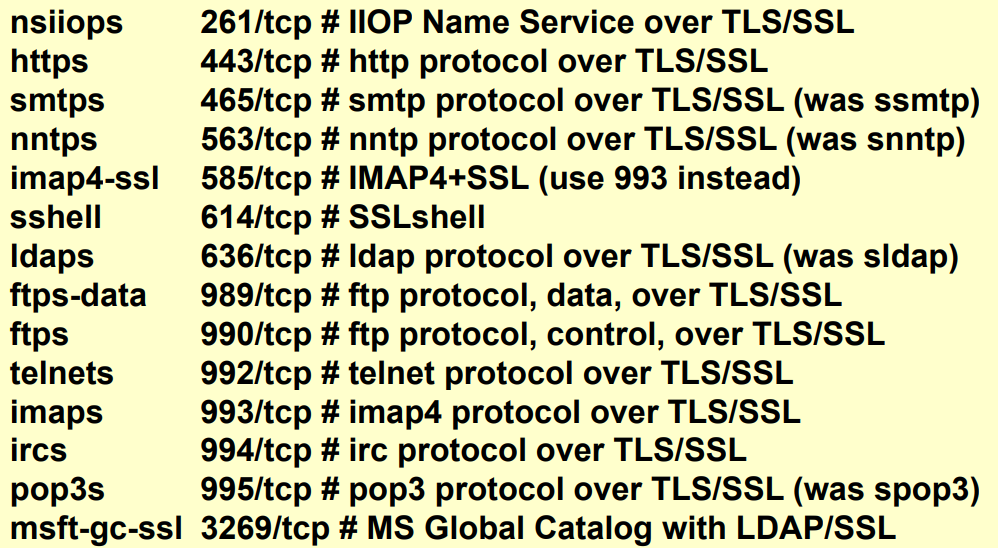
\includegraphics[width=0.4\textwidth]{/home/lorenzo/Notes/Information System Security/images/Screenshot from 2024-12-22 17-24-59.png}
    \caption{Official Ports for TLS/SSL Applications}
\end{figure}

\subsection{TLS - AuthN and Integrity}
\textbf{Peer AuthN} is performed \textbf{always at channel setup}:
\begin{itemize}
    \item The server must be authenticated (mandatory). Sends its public key (X.509 certificate) and responds to an implicit asymmetric challenge.
    \item The client can authenticate itself (optional): with public key, X.509 certificate and explicit challenge. 
\end{itemize}
For \textbf{authN} and \textbf{integrity} of \textbf{data}, TLS uses:
\begin{itemize}
    \item A Keyed-Digest (SHA-1 or better).
    \item An implicit MID to \textbf{avoid} Replay and Filtering attacks.
\end{itemize}
\subsection{TLS - Confidentiality}
\textbf{Data confidentiality} is granted by TLS in the following way:
\begin{enumerate}
    \item The client generates a session key used for symmetric encryption of data (using RC4, 3DES, IDEA, AES, or ChaCha20). 
    \item The session key is \textbf{exchanged} with the server via Asymmetric cryptography (using RSA or DH).
\end{enumerate}
\textcolor{red}{\textbf{N.B.}} Authentication is available in TLS 1.2, while is mandatory in TLS 1.3. 

\subsection{TLS Architecture}
\begin{minipage}{0.6\textwidth}
%	\vspace{-0.5cm}
    TLS is positioned \textbf{on top} of the transport layer (e.g TCP) and network layer (e.g. IP). 
    \begin{itemize}
        \item \textbf{Record protocol}: is positioned between TCP and the other TLS protocols and the various application protocol (e.g HTTP).
        \item \textbf{Handshake protocol}
        \item \textbf{Change Cipher Spec Protocol}: used to change the \texttt{algorithms}, \texttt{parameters} or \texttt{keys} on an already established TLS channel.
        \item \textbf{Alert Protocol}: used to send error information on the TLS channel before permanently closing it.
    \end{itemize} 
\end{minipage} 
\hspace{0.5cm}
\begin{minipage}{0.4\textwidth}
    \centering
    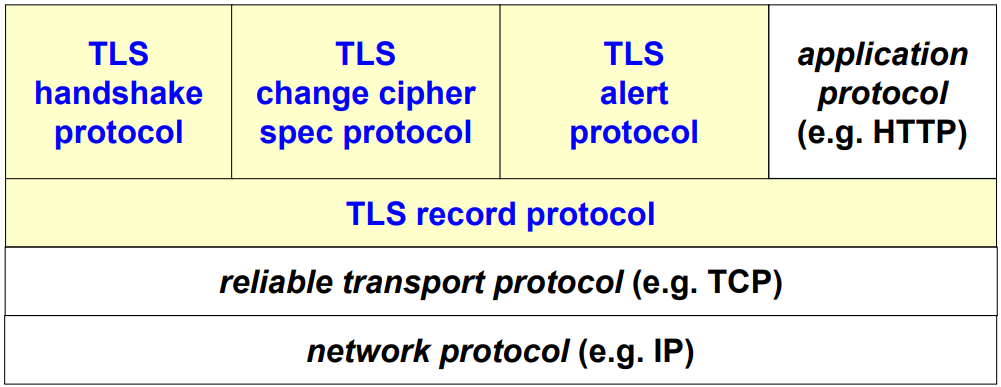
\includegraphics[width=\textwidth]{/home/lorenzo/Notes/Information System Security/images/Screenshot from 2024-12-23 09-45-39.png}
\end{minipage}

\subsection{TLS Handshake Protocol}
\begin{minipage}{0.6\textwidth}
%	\vspace{-0.5cm}
    The \textbf{Handshake Protocol} is used by TLS to perform \textbf{channel setup}, let's see an example:
    \begin{enumerate}
        \item The browser (\textbf{client} \textbf{C}) initiates a connection to the \textbf{web server} (\textbf{S}) by requesting the website
        (www.polito.it) over HTTPS.
        \item \textbf{C} and \textbf{S} discuss about the security configuration. They should both agree to use the \textbf{strongest common algorithms}.
        \item The \textbf{S} sends its certificate to \textbf{C} to prove its identity. The certificate includes the server’s public key and the domain name.\\
        3b) \textbf{S} will then respond to an Asymmetric CRA sent by the \textbf{C} (This is part of the handshake to confirm (implicitly)
        the server’s identity.)
        \item (Optional) \textbf{S} may require (explicitly) a client certificate to verify
        the user’s identity.
        \item \textbf{Key exchange} is performed. During this phase \textbf{C} and \textbf{S} exchange \textbf{master keys} that are linked to the session-ID. Every time a new \textbf{TLS Connection} is opened with that \textbf{session-ID}, a new connection oriented key must be generated by combining the master key and one of the previously exchanged random numbers. 
        \item Finally the \textbf{Secure TLS Channel} is opened and available to exchange data. 
    \end{enumerate}
\end{minipage} 
\hspace{0.1cm}
\begin{minipage}{0.5\textwidth}
    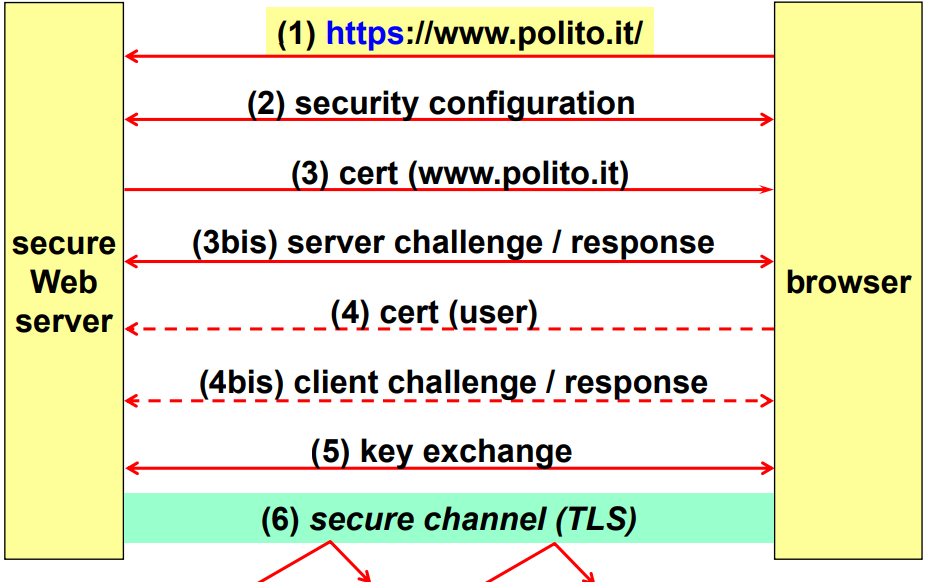
\includegraphics[width=0.9\textwidth]{/home/lorenzo/Notes/Information System Security/images/Screenshot from 2024-12-22 17-53-44.png}
\end{minipage}
\noindent
\\
\\
\\
After the Secure TLS Channel has been established, client and server will: 
\begin{itemize}
    \item Negotiate the \textbf{Session-ID}
    \item Exchange \textbf{random numbers} to be used for the subsequence generation of keys.
\end{itemize}
\subsection{TLS Session ID}
\begin{minipage}{0.6\textwidth}
%	\vspace{-0.5cm}
A typical web transaction involves the transmission of multiple elements between the client
(e.g., a web browser) and the server. To avoid the overhead of negotiating a new session for
each element (i.e. Many connections can be part of the same logical session), TLS uses a session
ID. \textbf{The session ID is a unique identifier that allows the client and server to resume a previous
session.}
If the client, when opening the TLS connection, sends a valid session-id, the negotiation
phase is skipped, and data can be immediately exchanged over the secure channel. \\
\textcolor{red}{\textbf{N.B.}} However, the client must start communicating in encrypted form; otherwise, the server will reject the
connection.
\end{minipage} 
\hspace{0.5cm}
\begin{minipage}{0.4\textwidth}
    \centering
    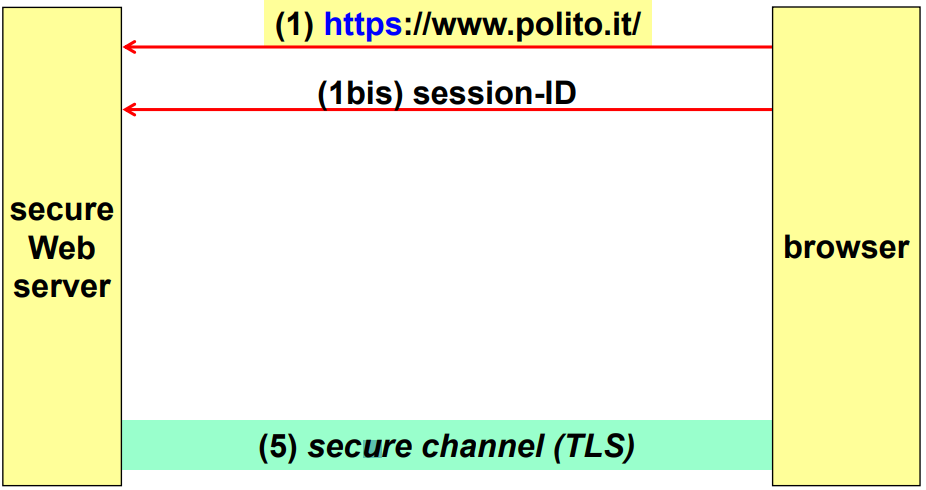
\includegraphics[width=\textwidth]{/home/lorenzo/Notes/Information System Security/images/Screenshot from 2024-12-23 10-01-33.png}
\end{minipage}
\begin{quotebox-red}{Beware}
    The server can reject the use of session-id (always or after a
    time passed after its issuance)
\end{quotebox-red} 

\subsection{TLS Session \textbf{\(\&\)}  Connections}
\begin{minipage}{0.6\textwidth}
%	\vspace{-0.5cm}
In TLS we have to distinguish the two:
\begin{itemize}
    \item \textbf{TLS Session}: it's a \textbf{logical association between client and server} created by the Handshake protocol. It defines a set of cryptographic parameters which are used during communication and can be shared by one or more TLS Connections (1:N).
    \item \textbf{TLS Connection}: it's a \textbf{transient} TLS Channel between client and server that is associated to one specific TLS Session (1:1).
\end{itemize}
\end{minipage} 
\hspace{0.5cm}
\begin{minipage}{0.4\textwidth}
    \centering
    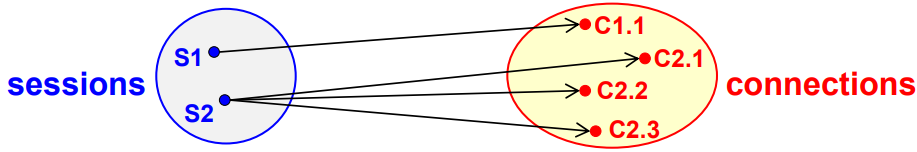
\includegraphics[width=\textwidth]{/home/lorenzo/Notes/Information System Security/images/Screenshot from 2024-12-23 10-17-23.png}
\end{minipage}

\subsection{Relationship among Keys and Sessions}
\begin{minipage}{0.6\textwidth}
%	\vspace{-0.5cm}
Every time we create a TLS session: we generate (with PKC) a \textbf{pre-master secret}. By generating the client random/server random value, we can mix them with the pre-master secret to generate the \textbf{master secret}, which is common to \textbf{all} the Connections of the Session. Each time we create a TLS Connection: we generate a \textbf{unique} client random/server random value. Combining them with the master secret we create \textbf{for this specific connetction and direction}:
\begin{itemize}
    \item Keys for MAC
    \item Keys for encryption
    \item IV for encryption
\end{itemize}
\end{minipage} 
\hspace{0.3cm}
\begin{minipage}{0.4\textwidth}
    \centering
    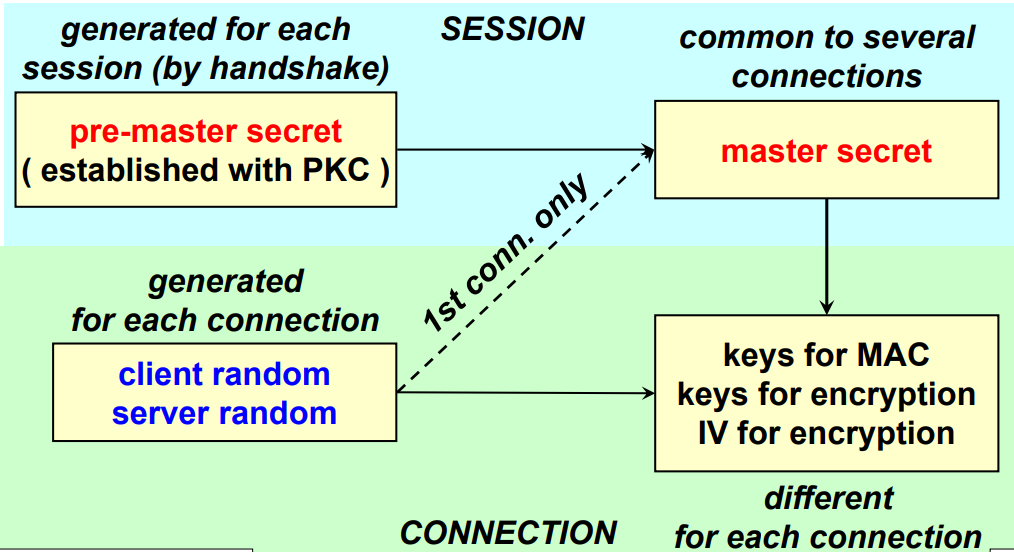
\includegraphics[width=\textwidth]{/home/lorenzo/Notes/Information System Security/images/Screenshot from 2024-12-23 15-57-51.png}
\end{minipage}

\subsection{TLS Record Protocol (authenticate-then-encrypt)}
The TLS Record Protocol secures application data during transmission.The steps:
\\
\begin{minipage}{0.6\textwidth}
\vspace{0.5cm}
\begin{enumerate}
\item \textbf{Fragmentation}: Divides the data (from the application layer or higher-level TLS protocols) into smaller blocks or "records" that can be transmitted efficiently.
\item The fragmented data is \textbf{compressed} (\textbf{Optionally}).
\item Ma MAC is computed over the data (\(\rightarrow\) to verify integrity and authenticity of the data).
\[ 
\hspace{-0.8cm}
MAC = message\_digest(key,seq_number\ ||\ type\ ||\ version\ ||\ length\ ||\ fragment)
\]
There are two different keys: the sender-write-key  and the receiver-write-key. This separation prevents replay attack.

\end{enumerate}
\end{minipage} 
\hspace{0.9cm}
\begin{minipage}{0.4\textwidth}
    \centering
    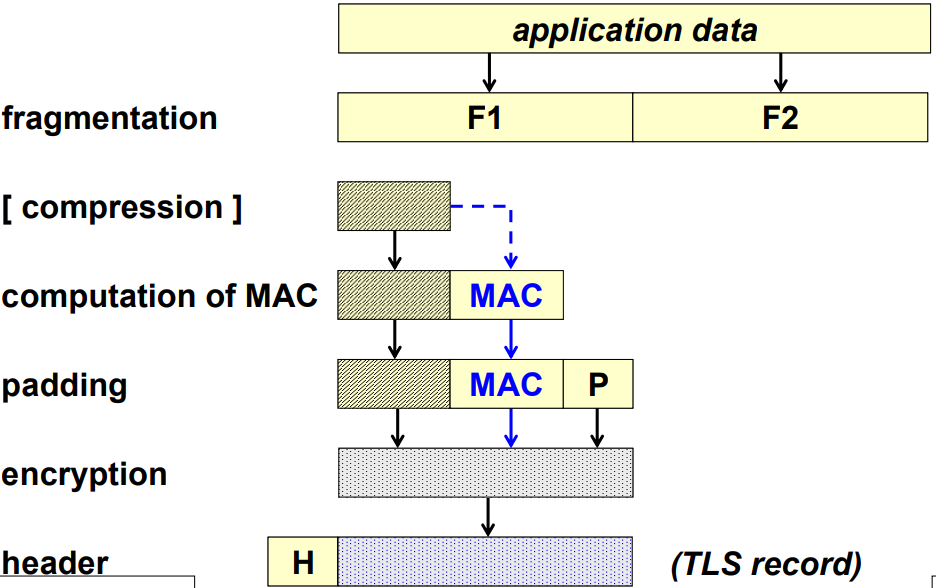
\includegraphics[width=\textwidth]{/home/lorenzo/Notes/Information System Security/images/Screenshot from 2024-12-23 10-29-46.png}
\end{minipage}

\begin{quotebox-grey}{Replay attack}
    \begin{minipage}{0.6\textwidth}
    %	\vspace{-0.5cm}
    \begin{itemize}
        \item The sender (Client) sends an encrypted command, like Transfer \$100 to the receiver (Server).
        \item An attacker intercepts this message and replays the exact encrypted data back to the sender (Client).
        \item Since the sender and receiver share the same key, the sender would decrypt the message and potentially act on it (depending on the system design), causing confusion or security breaches.
    \end{itemize}
    
    \end{minipage} 
    \hspace{0.3cm}
    \begin{minipage}{0.4\textwidth}
        \centering
        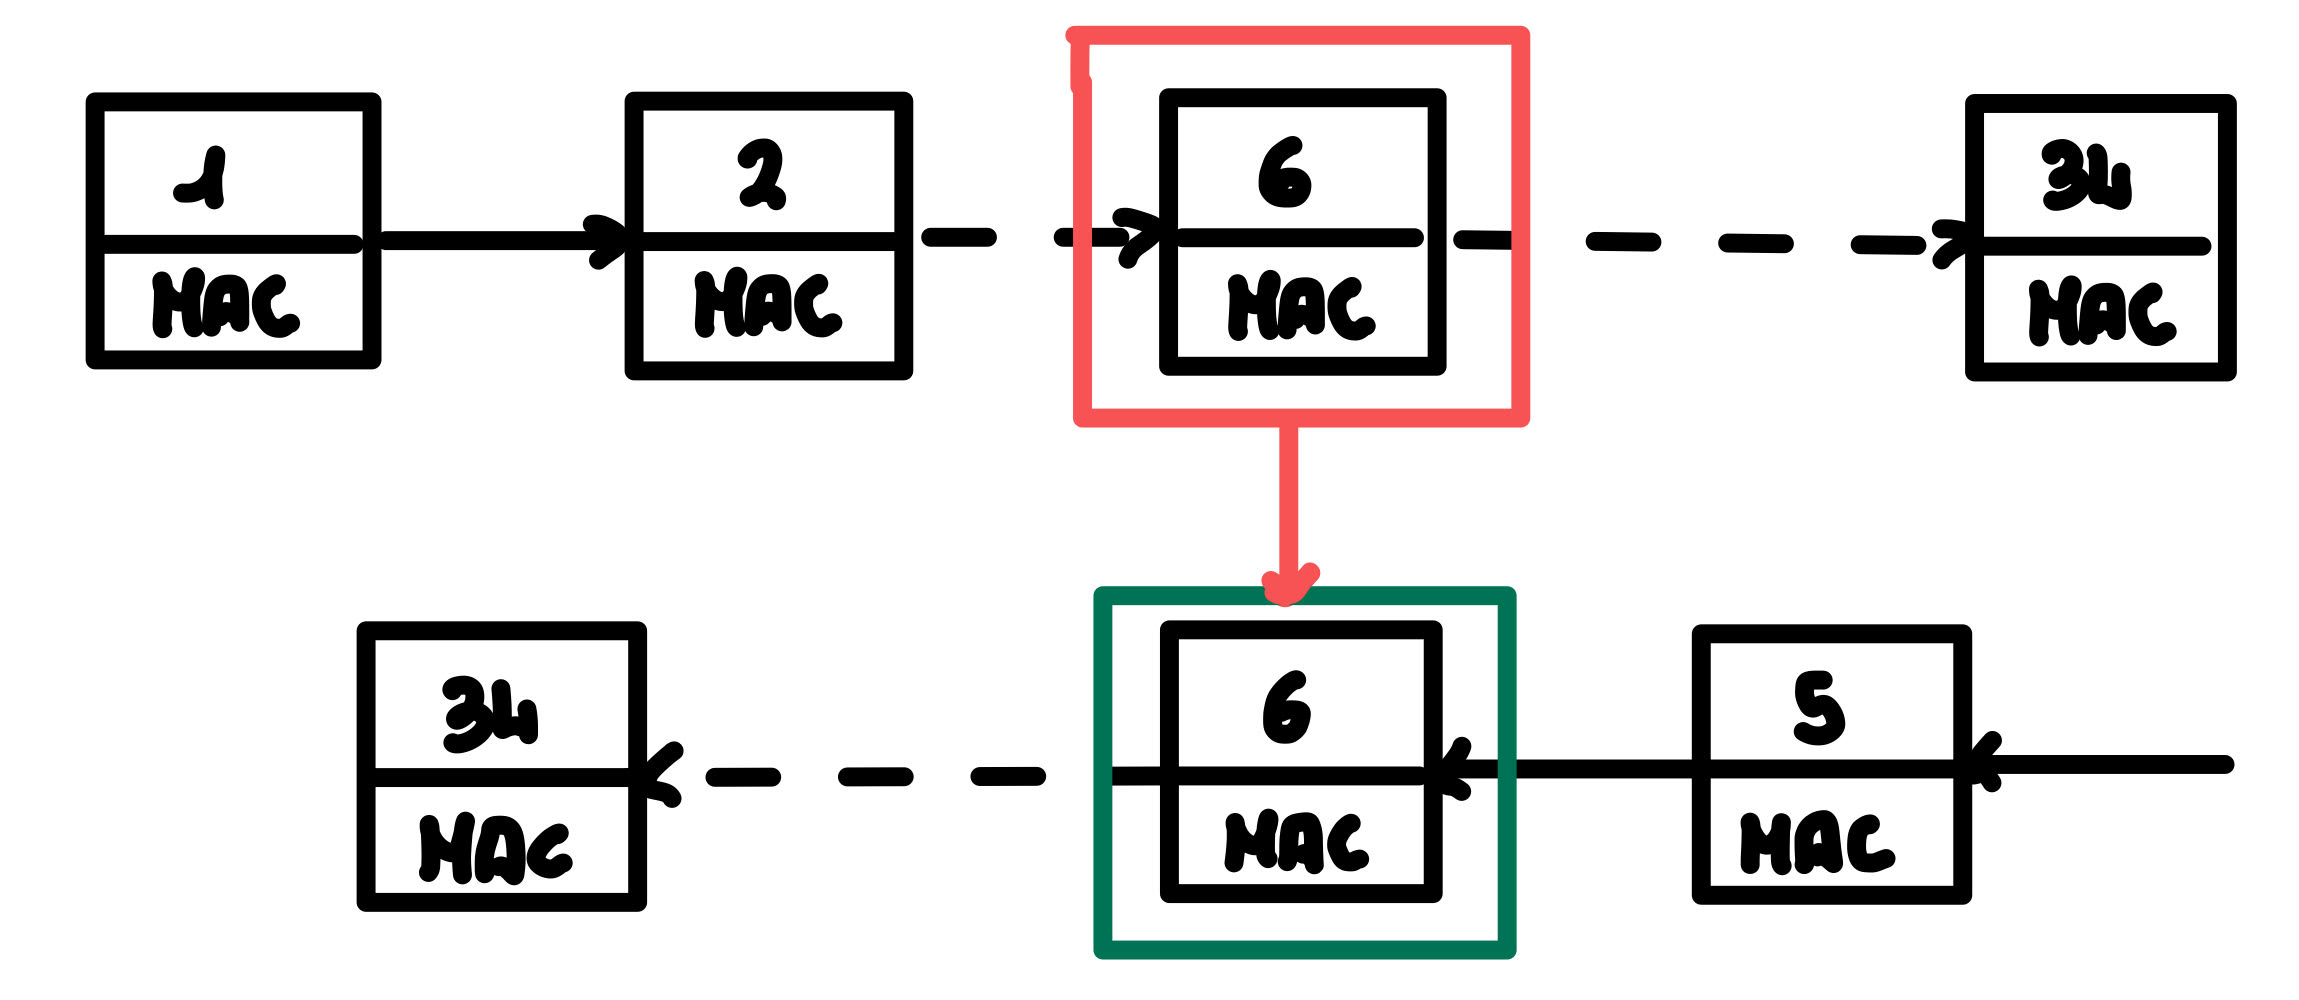
\includegraphics[width=0.9\textwidth]{/home/lorenzo/Notes/Information System Security/images/image.png}
    \end{minipage}

\end{quotebox-grey}
\begin{enumerate}
\setcounter{enumi}{3}
\item \textbf{Padding} is added to make data 
encryptable.
\item Data is \textbf{encrypted}. Steps:
\\
\begin{minipage}{0.5\textwidth}
	
\begin{itemize}
    \vspace{-1cm}
    \item \textbf{Generation of MAC}: the (compressed) data is combined with the MAC key and sequence of number as explained before. 
    \item \textbf{Symmetric Encryption}: takes (data || MAC || padding), and, by using the IV and the encryption key, generates the protected data.
\end{itemize}
\end{minipage} 
\hspace{0.5cm}
\begin{minipage}{0.4\textwidth}
    \centering
    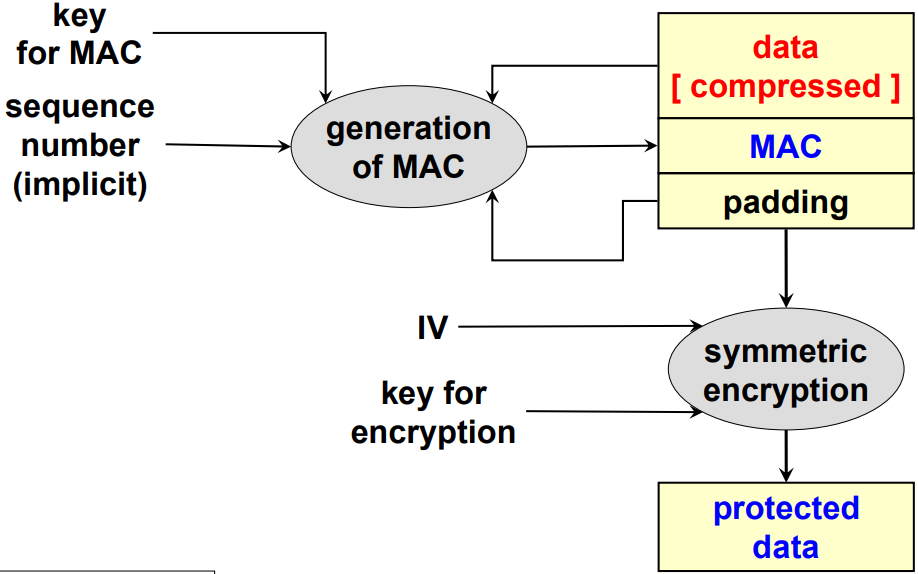
\includegraphics[width=0.9\textwidth]{/home/lorenzo/Notes/Information System Security/images/Screenshot from 2024-12-23 15-09-45.png}
\end{minipage}

\item The encrypted data is packaged into a TLS record (header+payload).
\end{enumerate}

\subsection{Perfect Forward Secrecy}
If a server has a certificate valid for both signature and encryption, it can be used bot for authN (via Signature) and Key Exchange (Asymmetric Encryption of the Session Key). If an attacker copies all the encrypted traffic and later discovers the server's SK, the attacker can decrypt all traffic (\textbf{past}, \textbf{present} and \textbf{future}).\\
\textbf{Perfect Forward Secrecy} is a technique in which: if a PK/SK pair is compromised, only the \textbf{present} and \textbf{future} traffic can be decrypted.\\
This mechanism (implemented in TLS) is achieved through the use of \textbf{ephemeral keys} (temporary keys) that are generated for each session and are not stored. For \textbf{authenticity}, the one-time key must be signed (the server’s SK is only used for signing, granting server authN). However, it cannot have an associated X.509 certificate, as the CA process is slow and often not available online. "Ephemeral" mechanisms are:
\begin{itemize}
    \item Suitable for DH (Diffie-Helmann).
    \item Slow for RSA \(\rightarrow\) a compromised would be to re-use N times the same key. 
\end{itemize}
This means that with Perfect Forward Secrecy:
\begin{itemize}
    \item If the \textbf{short term SK} is compromised \(\rightarrow\) the attacker can decrypt \textbf{only the present and future} (typically only for the session) traffic.
    \item If the \textbf{long term SK} is compromised \(\rightarrow\) the server can \textbf{no longer perform authN} but at least the attacker cannot decrypt any traffic. 
\end{itemize}
\begin{quotebox-grey}{Example}
ECDHE (Elliptic Curve Diffie-Helmann Ephemeral) is a key exchange protocol that provides PFS.
\end{quotebox-grey}

\subsection{TLS Downgrade Attack}
When the client negotiates with the server which version of TLS to use: 
\begin{itemize}
    \item The client always send (in \texttt{Client Hello}) the \textbf{highest supported version}.
    \item The server notifies (in \texttt{Server Hello}) the version to be used, which must be the highest in common.
\end{itemize}
An attacker could send fake server response, forcing a version downgrade until a vulnerable one is reached, and then execute an attack. 
\begin{quotebox-red}{Beware}
Initial messages, before the setup of the secure channel, are not protected by the security protocol. 
\end{quotebox-red}
\noindent
This behaviour does not (always) mean that we are under attack, it could be simply a \textbf{Insecure downgrade} (\(\rightarrow\) Some servers do not send the correct response, rather they close the connection. Then the client has no choice to try again with a lower protocol version).

\section{Virtual Servers and TLS}
\textcolor{red}{\textbf{Problem:}} the \textbf{Virtual Servers problem} is very frequent with \textbf{web hosting}: different logical names are associated to the \textbf{same IP address} (e.g.: \texttt{home.myweb.it=1.2.3.4} and \texttt{food.myweb.it=1.2.3.4}).\\
This problem is easily solved in \textbf{HTTP/1.1}: the client uses \textbf{Host header} to specify the Logical Name of the server it want to connect to. \\
But it is a problem for HTTPS, where the domain name is encrypted (because
TLS, transport layer security protocol, is activated before HTTP, application layer protocol).\\
\\
\textcolor{green}{\textbf{Solutions:}}
\begin{itemize}
    \item Collective (wildcard) certificates: the private key is shared by all servers. e.g. \texttt{*.myweb.it}.
    Different browsers may react differently to this solution.
    \item Certificate with a list of servers in the SAN (subjectAltName) field: The private key is
    shared among all servers, and the certificate needs to be reissued whenever a server is
    added or removed.
    \item The SNI (Server Name Indication) extension: The client sends the domain name in the
    initial message. The server can then choose the correct certificate. Limited support by browsers and servers.
\end{itemize}
\section{ALPN extension (Application-Layer Protocol Negotiation)}
The \textbf{ALPN extension} was created to \textbf{speed up} connection creation by avoiding negotiation \texttt{round-trips}. ALPN works in the following way:
\begin{itemize}
    \item (ClientHello) ALPN = true + list of supported application protocols;
    \item (ServerHello) ALPN = true + selected application protocols;
\end{itemize}
\textcolor{red}{\textbf{N.B.}} It is particularly important to negotiate HTTP/2 and QUIC, since (for example)
Chrome and Firefox support HTTP/2 only over TLS.
\begin{quotebox-yellow}{}
    ALPN is useful also for those servers that use different certificates for the different application
    protocols.
\end{quotebox-yellow}

\section{TLS Fallback - Signaling Cipher Suite Value}
The \textbf{SCSV estension} is used to prevent protocol downgrade attacks. SCSV works in the following way:
\begin{itemize}
    \item When a connection to a server is closed during the Handshake protocol negotiation
    phase, the client (upon opening downgraded connection) should send to the server a
    new (dummy) ciphersuite called \textbf{TLS\_FALLBACK\_SCSV};
    \item Upon receiving TLS\_FALLBACK\_SCSV and a version lower then the highest one supported, the server must send a new Fatal Alert value: "inappropriate\_fallback".\\
    \\
    Immediately after sending this value, the \textbf{TLS channel is closed} \(\rightarrow\) the client should
    retry with its highest protocol version;
\end{itemize}
\textcolor{red}{\textbf{N.B.}} However, many servers do \textbf{not} support SCSV, but at least \textbf{most} of them have fixed this bad behaviour \(\rightarrow\) browsers can \textbf{disable insecure downgrade}.

\section{DTLS (Datagram Transport Layer Security)}
\textbf{DTLS} tries to apply the concepts of TLS to \textbf{datagram security} (e.g. UDP). It does not
offer the same security properties as TLS and is in competition with IPsec and Application Security.\\
For example, if we use \textbf{SIP} (\textbf{Session Initiation Protocol}) we could implement security with:
\begin{itemize}
    \item IPsec
    \item TLS (SIP over TCP)
    \item DTLS (SIP over UDP)
    \item Secure SIP
\end{itemize}

\section{HTTP Security}
In\textbf{HTTP/1.0} some \textbf{bad security mechanisms} are defined:
\begin{itemize}
    \item \textbf{Address-based Access Control}: performed by the server on the IP address of client. 
    \item \textbf{Password-based Access Control}: \textbf{username} and \textbf{password} are sent encoded (base64).
\end{itemize}
Both of them are \textbf{highly insecure} since HTTP assumes we are using a Secure Channel. 
\begin{quotebox-yellow}{}
From HTTP/1.1 \textbf{digest authN} based on Symmetric CRA was introduce.
\end{quotebox-yellow}

\subsection{HTTP Basic Authentication}
\begin{minipage}{0.5\textwidth}
%	\vspace{-0.5cm}
    \begin{enumerate}
        \item After having created the channel using \textbf{HTTP/1.0}, the server automatically responds
        with an "authentication failed" message but does \textbf{not} close the channel, because the client (maybe) did not know that authN was needed \(\rightarrow\) the servers sends an \textbf{authN request} to the client;
        \item The client's browser will open a pop-up that asks the client to enter its credentials in order to perform authN.
        \item The client submits its credentials encoded in Base64 (\textbf{not encrypted} \(\rightarrow\) \textbf{no secure}).
        
            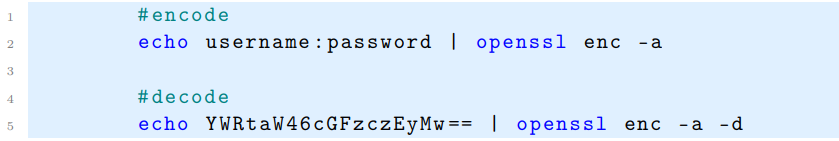
\includegraphics[width=0.9\textwidth]{/home/lorenzo/Notes/Information System Security/images/Screenshot from 2024-12-24 11-31-43.png}

        \item The server can \textbf{verify} the credentials and (eventually) send the information requested by the client. 
    \end{enumerate}
\end{minipage} 
\hspace{0.2cm}
\begin{minipage}{0.5\textwidth}
    \centering
    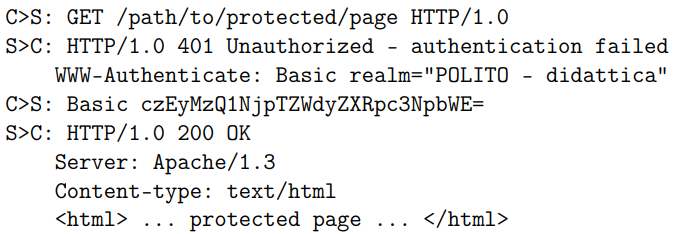
\includegraphics[width=1.1\textwidth]{/home/lorenzo/Notes/Information System Security/images/Screenshot from 2024-12-24 11-29-20.png}
\end{minipage}

\subsection{HTTP Digest Authentication}
The keyed-digest introduced in \textbf{HTTP/1.1} is computed in the following way:
\begin{figure}[h]
    \centering
    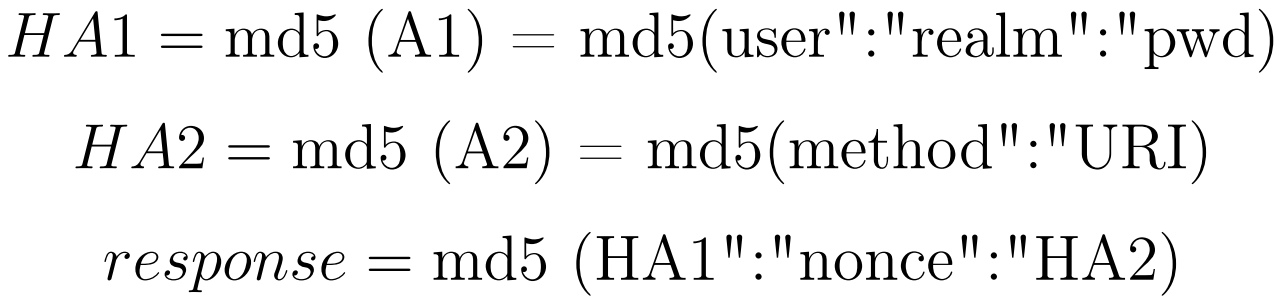
\includegraphics[width=0.4\textwidth]{/home/lorenzo/Notes/Information System Security/images/Screenshot from 2024-12-24 11-52-15.png}
\end{figure}
\noindent
\begin{itemize}
    \item The sever may even insert an \textbf{"opaque"} field to send some state information to the client.
    \item The server uses a nonce to prevent replay attacks.
\end{itemize}


\begin{minipage}{0.5\textwidth}
%	\vspace{-0.5cm}
    \begin{enumerate}
        \item After having created the channel using \textbf{HTPP/1.1}, the server \textbf{automatically} responds with a "\texttt{Authentication failed}" message but \textbf{not} close the channel, because the client maybe did \textbf{not} know that authN was needed, so the server sends an \textbf{authN request} to the client containing the \textbf{nonce} and the \textbf{opaque} values encoded in Base64.
        \item The clint's browser will open a pop-up that asks the client to perform authN \(\rightarrow\) the client computes the keyed-digest and sends it, together with the \textbf{opaque}, to the server. 
        \item The server can then \textbf{verify} the credentials and (eventually) send the information request by the client.
    \end{enumerate} 
\end{minipage} 
\hspace{0.3cm}
\begin{minipage}{0.5\textwidth}
    \centering
    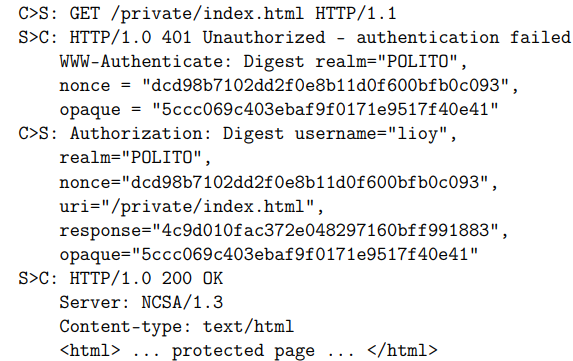
\includegraphics[width=\textwidth]{/home/lorenzo/Notes/Information System Security/images/Screenshot from 2024-12-24 12-05-23.png}
\end{minipage}

\newpage
\subsection{HTTP \& TLS/SSL}
We can use both HTTP and TLS/SSL by activating them in one of the following orders:
\begin{itemize}
    \item \textbf{TLS then HTTP}: the client connects to the server using TLS and then sends the HTTP request (\(\rightarrow\) Content inspection is not possible!).
    \item \textbf{HTTP then TLS}: the client connect to the server using HTTP and then upgrades the connection to TLS (\(\rightarrow\) We see the HTTP methods until the upgrade!).
\end{itemize}
\begin{quotebox-red}{Beware}
They are \textbf{not} equivalent as the activation order has an impact over \texttt{applications}, \texttt{firewall} and IDS.
\end{quotebox-red}
In general the most used approach is "TLS then <proto>" (e.g. HTTPS).

\begin{customquote}
\vspace{-0.4cm}
\subsubsection{TSL AuthN at the Application Layer}
Via client authentication it’s possible to identify the user that opened the channel (without asking for his username and password).\\
The identification process of a client can be done at the application level, but it is not a
standard feature of TLS.
\end{customquote}

\begin{customquote}
\vspace{-0.4cm}
\subsubsection{AuthN in Web applications}
\begin{quotebox-yellow}{}
The \textbf{earlier} access control is performed, the \textbf{smaller} is the attack surface.
\end{quotebox-yellow}
\begin{minipage}{0.4\textwidth}
\vspace{-1cm}
Moreover, there is no need to repeat authentication across different parts of the application if the user's identity is securely propagated throughout the application. Some web servers support a (semi-)automatic mapping 
between the credential extracted from the X.509 certificate and the users of the HTTP service and/or the OS.
\end{minipage} 
\hspace{0cm}
\begin{minipage}{0.5\textwidth}
    \centering
    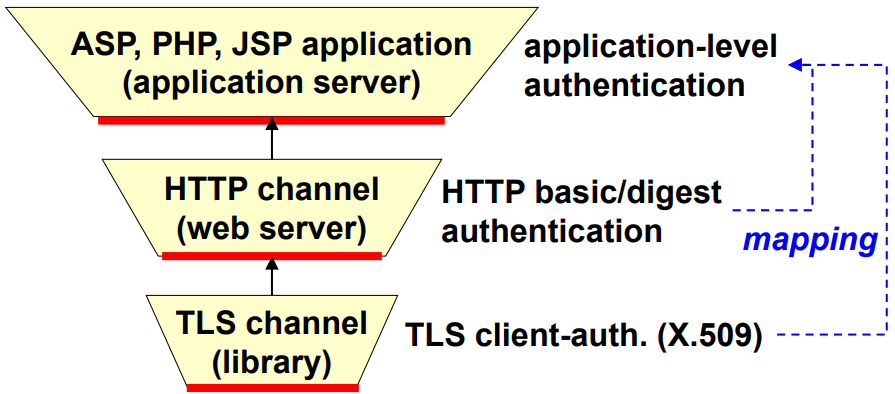
\includegraphics[width=1.1\textwidth]{/home/lorenzo/Notes/Information System Security/images/Screenshot from 2024-12-26 10-52-14.png}
\end{minipage}
\end{customquote}

\begin{customquote}
\vspace{-0.4cm}
\subsubsection{Web Form Security}
Technically speaking, the security of the page containing the form is not important (e.g. http://www.ecomm.it/login.html). The actual security depends on the URI of the method used to send the data to the server (e.g <form … action=“https://www...>).
Yet, as a form of psychological help for the users, we should also look to implement security in the page containing the form
\end{customquote}

\section{HTTP Strict Transport Security (HSTS)}
The \textbf{HSTS extension} is used by HTTP server to declare that its interaction with \textbf{User Agent} (\textbf{UA} \(\rightarrow\) e.g. browser, etc...) \textbf{must only be via HTTPS}, effectively preventing Protocol Downgrade and Cookie Hijacking attacks.\\ HSTS is applied \textbf{only} upon receiving a \textbf{valid HTTPS response}. Its validity is renewed at every access and it may:
\begin{itemize}
    \item Include subdomains (recommended).
    \item Be pre-loaded into the servers.
\end{itemize}
\begin{quotebox-grey}{Syntax}   
\begin{minipage}{0.4\textwidth}
    The syntax is:
    \begin{center}
        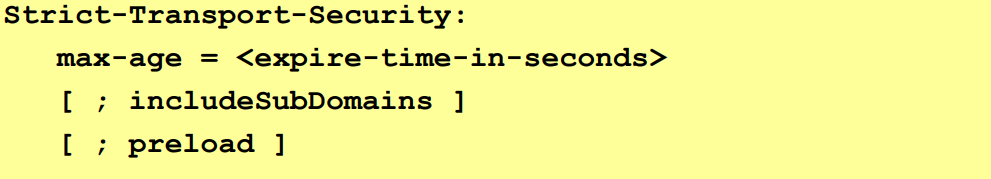
\includegraphics[width=1.1\textwidth]{/home/lorenzo/Notes/Information System Security/images/Screenshot from 2024-12-26 11-24-04.png}  
    \end{center}
\end{minipage} 
\hspace{1cm}
\begin{minipage}{0.4\textwidth}
    \textbf{Example:}
    \begin{center}
        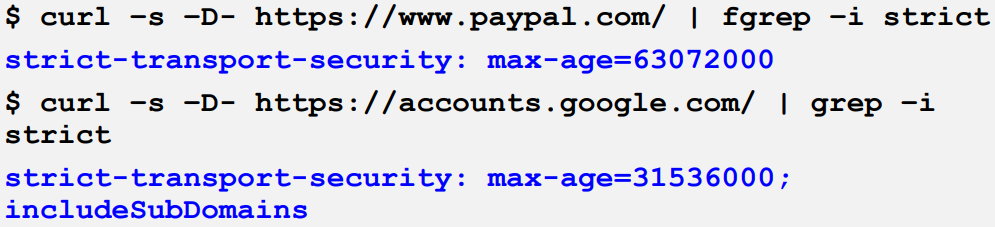
\includegraphics[width=1.1\textwidth]{/home/lorenzo/Notes/Information System Security/images/Screenshot from 2024-12-26 11-48-14.png} 
    \end{center} 
\end{minipage}
\newline
\\
Upon receiving an answer from the server that will contain the \textbf{HSTS Header}, inside there will be specified:
\begin{itemize}
    \item The expiration data in seconds.
    \item (Optionally) the subdomains.
    \item (Optionally) the option of being added to the client's pre-load list.
\end{itemize}
\end{quotebox-grey}

\subsection{HTTP Public Key Pinning (HPKT)}
\begin{minipage}{0.7\textwidth}
%	\vspace{-0.5cm}
The \textbf{HPKP extension} is used by HTTP servers to declare that it is using a certain \textbf{PK} by specifying the Digest of the PK and/or one or more CAs in its chain (except the root CA). The User Agent (UA) caches this key and will refuse to connect to a site presenting a different key. 
\end{minipage} 
\hspace{0.3cm}
\begin{minipage}{0.3\textwidth}
    \centering
    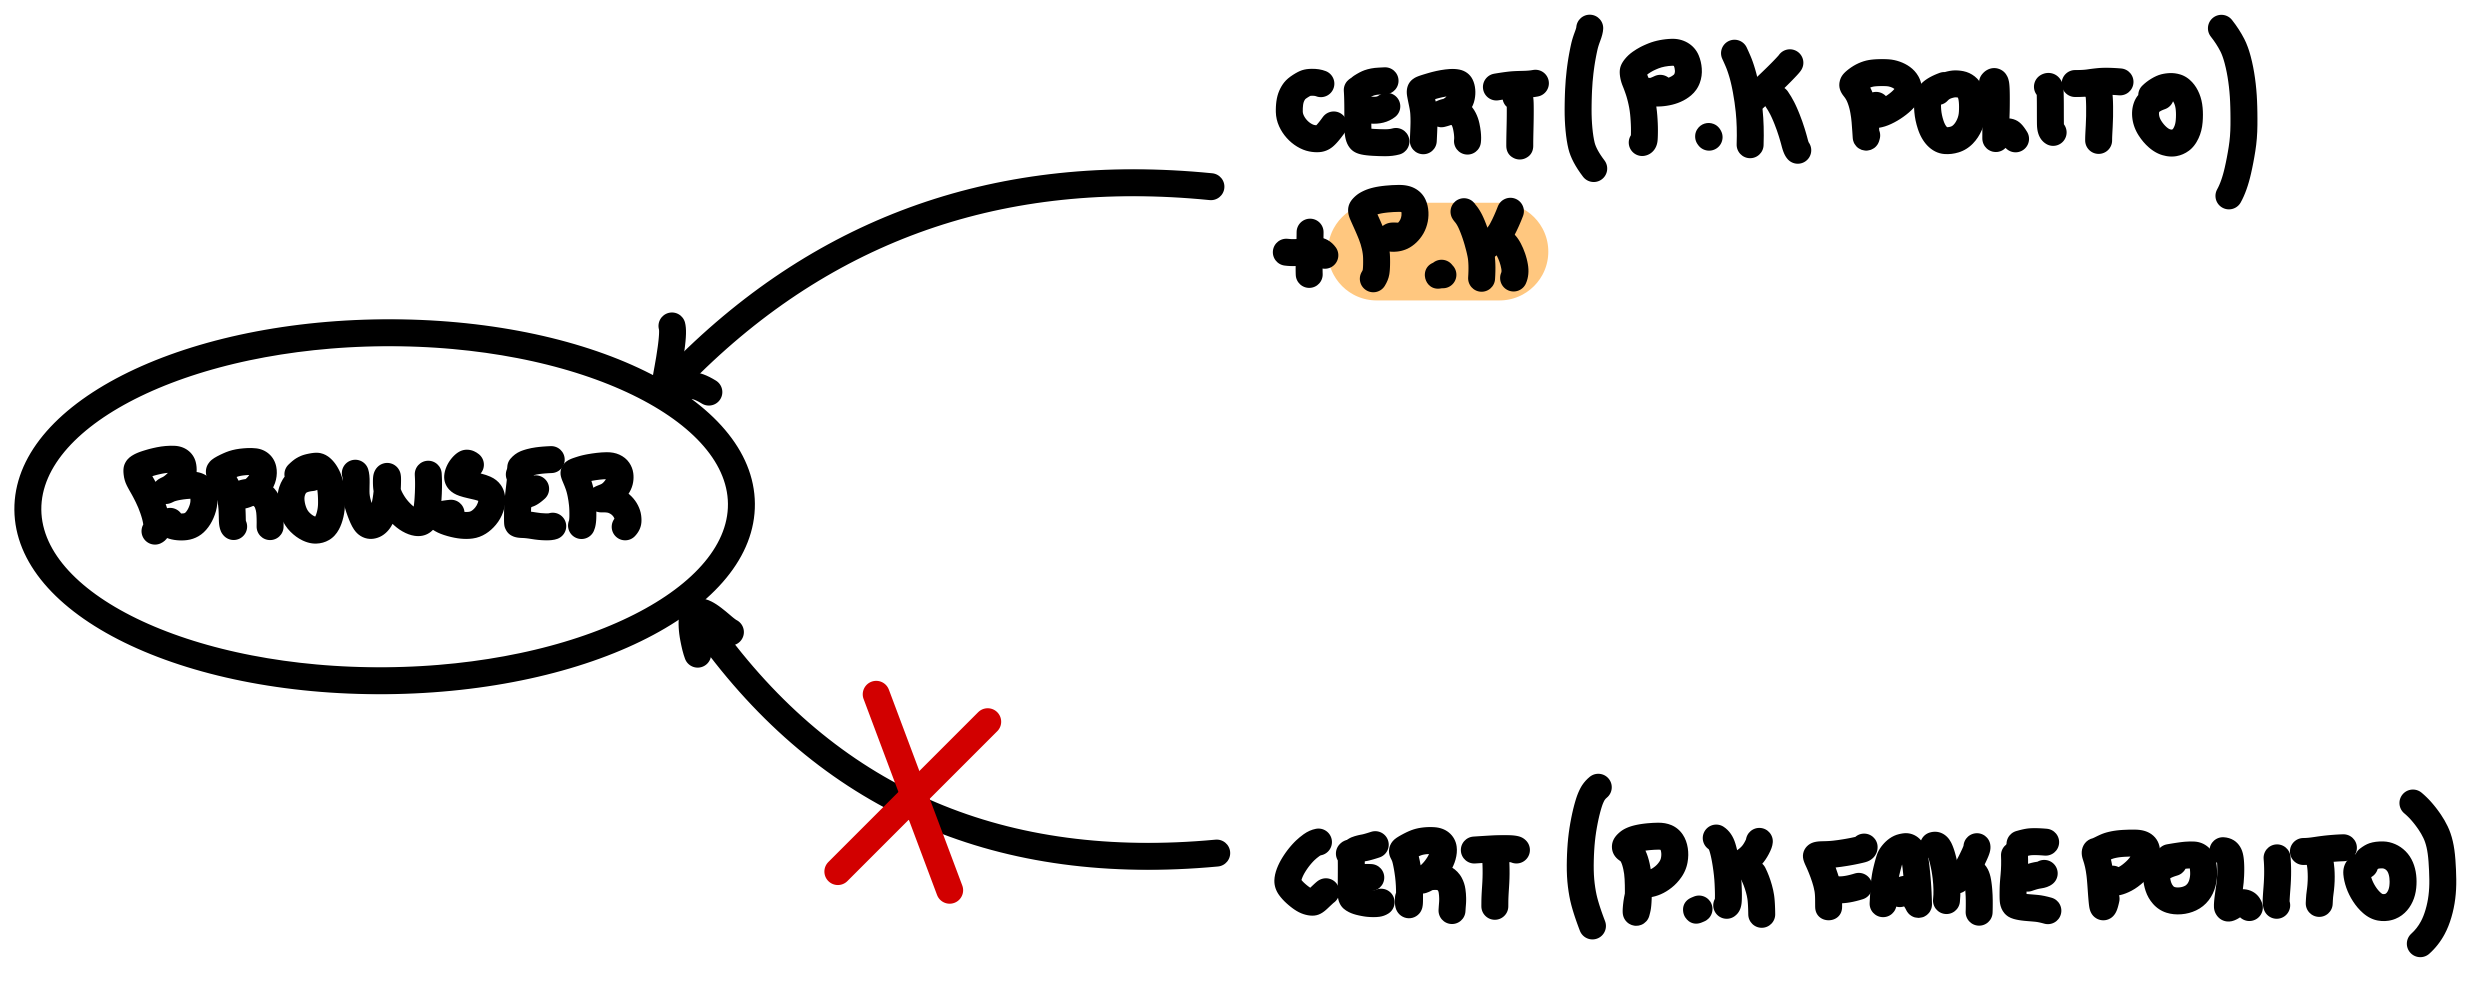
\includegraphics[width=0.7\textwidth]{/home/lorenzo/Notes/Information System Security/images/image copy.png}
\end{minipage}

\begin{itemize}
    \item HPKP is a \textbf{TOFU} (\textbf{Trust On First USe}) technique.
    \item HPKP is dangerous if we lose control of the key.
    \item HPKP can cause problems with key updates \(\rightarrow \) always include a backup key.
\end{itemize}
\begin{quotebox-grey}{Syntax}
    \begin{minipage}{0.4\textwidth}
    \vspace{-0.5cm}
        The syntax is:
        \begin{center}
            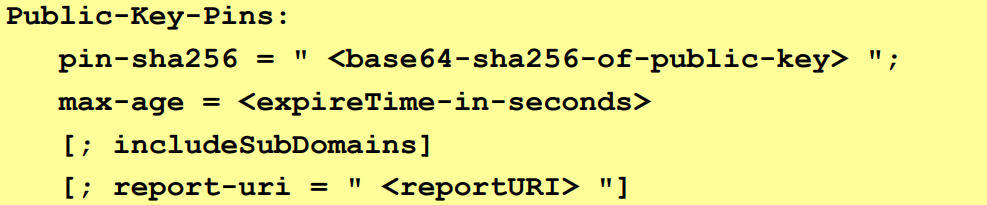
\includegraphics[width=1.1\textwidth]{/home/lorenzo/Notes/Information System Security/images/Screenshot from 2024-12-26 12-31-44.png} 
        \end{center} 
        %\vspace{1cm}
        \begin{center}
            \includegraphics[width=1.1\textwidth]{/home/lorenzo/Pictures/Screenshots/Screenshot from 2024-12-26 12-33-07.png} 
        \end{center}
        
    \end{minipage} 
    \hspace{1cm}
    \begin{minipage}{0.4\textwidth}
        \textbf{Example}
        \begin{center}
        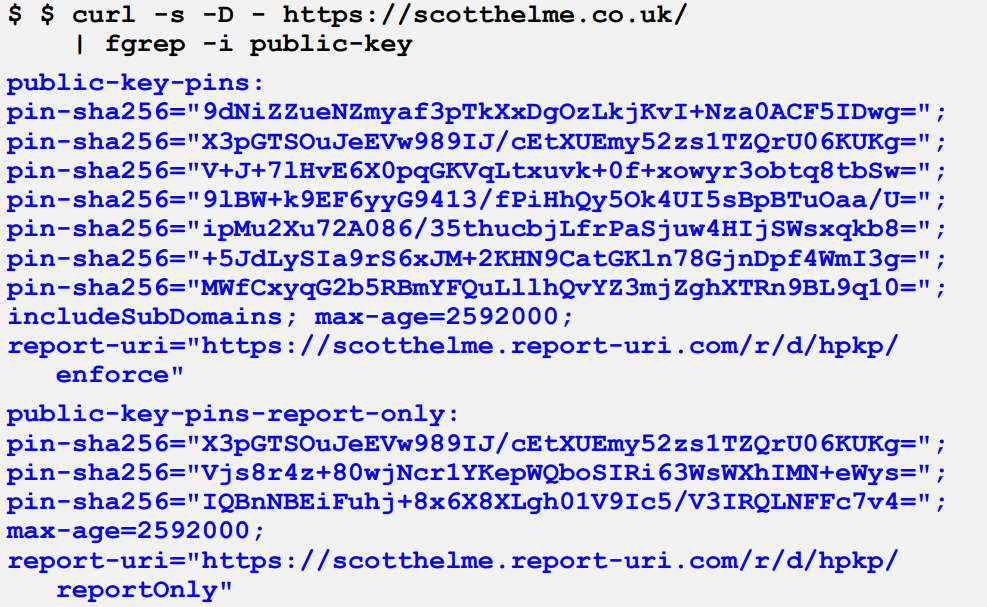
\includegraphics[width=1.1\textwidth]{/home/lorenzo/Notes/Information System Security/images/image copy 2.png}
        \end{center}
    \end{minipage}
    \noindent
    \\
    The \textbf{HPKP Header} includes:
    \begin{itemize}
        \item The digest of the PK computed with SHA-256.
        \item The expiration date in seconds.
        \item (Optionally) the subdomains.
        \item (Optionally) the report URI that is used to report violations.
    \end{itemize}
    \textcolor{red}{\textbf{N.B.}} HPKP can work in \textbf{enforcing} or \textbf{report-only mode}.
\end{quotebox-grey}

\noindent{\color{gray!50}\rule{\textwidth}{0.5pt}}
%---------------------------------
\section{E-Payment System}
What happen in the past:
\begin{itemize}
    \item Failure of digital cash due to technical and legal reasons.
    \item Failure of a dedicated payment protocol. (SET-Secure Electronic Transaction) caused by technical and organizational challenges.
    \begin{quotebox-red}{Beware}
    Providing users with specialized software can compromise the security of the system. 
    \end{quotebox-red}
\end{itemize}
Currently, the most widely used approach is transmitting credit card numbers over a TLS channel. However, this does not guarantee protection against fraud: in the past, VISA Europe reported that internet transactions accounted for about 50\% of fraud attempts, despite representing only 2\% of total transactions.

\newpage
\subsection{Web-Based Payment Systems}
The steps are:
\\
\\
\begin{minipage}{0.6\textwidth}
%	\vspace{-0.5cm}
    \begin{enumerate}
        \item The \textbf{merchant M} presents the products or services on their website for the \textbf{carholder C} to browser. 
        \item \textbf{C} places an order through the merchant's website, initiating the payment process.
        \item \textbf{M} redirects \textbf{C} to a \textbf{payment gateway PG}.
        \item \textbf{PG} will create a \textbf{Secure TLS channel} between the \textbf{PG} itself and \textbf{C}.
        \item \textbf{C} provide the credit card data.
        \item Inside the \textbf{PG}, a \textbf{Virtual POS (Point Of Sale)} will handle the data and will ask to the payment network (of the specific credit card) if they are valid.
        \item If the provided credit card data are correct, the payment network will return a
        positive answer.
        \item Finally \textbf{M} is informed of the confirmation of the transaction and it will provide the goods to \textbf{C}.
    \end{enumerate} 
\end{minipage} 
\hspace{0.3cm}
\begin{minipage}{0.4\textwidth}
    \centering
    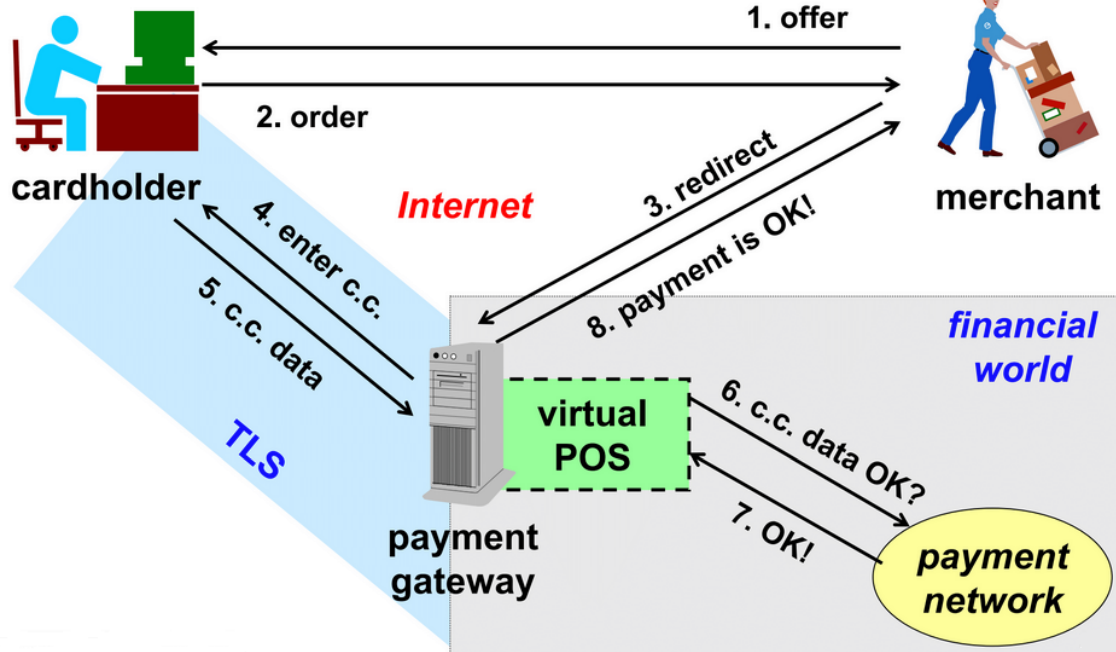
\includegraphics[width=\textwidth]{/home/lorenzo/Notes/Information System Security/images/Screenshot from 2024-12-26 14-27-18.png}
\end{minipage}
\noindent
\\
\\
\\
Different \textbf{PG} can have different \textbf{deduction fees} (e.g 5\%,10\%,etc...) which cumulates with the price proposed by \textbf{M}.\\
In order for all of this work, \textbf{C must have TLS enabled} in its browser. 
\begin{quotebox-grey}{Consequences}
\begin{itemize}
    \item The effective security depends upon the configuration of both the server and the client.
    \item The \textbf{PG} has all the information (payment + goods) while \textbf{M} knows only info about the goods.
\end{itemize}
\end{quotebox-grey}

\subsection{PCI DSS (Payment Card Industry Data Security Standard)}
The \textbf{PCI DSS} standard is required by \textbf{all credit issuers} or internet-based transactions. It contains very detailed technical prescriptions (compared to other security standards):
\begin{itemize}
    \item \textbf{Design, Build and Operate a Protected Network:}
    \begin{itemize}
        \item \textbf{R1}:install and maintain a configuration with a firewall to protect access to cardholders’ data.
        \item \textbf{R2}: do not use pre-defined system passwords or other security parameters set by
        the manufacturer.
    \end{itemize}
    \item \textbf{Protect the Cardholders’ Data:}
    \begin{itemize}
        \item \textbf{R3}: protect the stored cardholders’ data.
        \item \textbf{R4}: encrypt the cardholders’ data hen transmitted across an open public network.
    \end{itemize}
    \item \textbf{Establish and Follow a Program For Vulnerability Management:}
    \begin{itemize}
        \item \textbf{R5}: use an antivirus and regularly update it.
        \item \textbf{R6}: develop and maintain protected applications and systems.
    \end{itemize}
    \item \textbf{Implement Strong Access Control:}
    \begin{itemize}
        \item \textbf{R7}: limit the access to the cardholders’ data only to those needed for a specific risk.
        \item \textbf{R8}: assign a single unique ID to each user.
        \item \textbf{R9}: limit physical access to the cardholders’ data.
    \end{itemize}
    \item \textbf{Regularly Monitor and Test the Networks:}
    \begin{itemize}
        \item \textbf{R10}: monitor and track all accesses to the network resources and cardholders’ data.
        \item \textbf{R11}: periodically test the protection systems and procedures.
    \end{itemize}
    \item \textbf{Adopt a Security Policy:}
    \begin{itemize}
        \item \textbf{R12}: adopt a security policy.
    \end{itemize}
\end{itemize}